Selain meningkatkan keselamatan navigasi, metode yang diusulkan juga perlu dievaluasi dari sisi efisiensi pergerakan robot. Pada sistem navigasi robot bergerak, peningkatan margin keselamatan sering kali diikuti oleh konsekuensi berupa penambahan waktu tempuh atau perubahan karakteristik lintasan karena robot mempertahankan jarak yang lebih besar terhadap obstacle. Oleh karena itu, efisiensi navigasi pada penelitian ini dievaluasi menggunakan dua metrik utama, yaitu waktu tempuh (\textit{traversal time}) dan panjang lintasan (\textit{path length}).

\subsection{Analisis Waktu Tempuh}

Waktu tempuh menunjukkan durasi yang dibutuhkan robot untuk bergerak dari posisi awal menuju titik tujuan. Nilai ini merepresentasikan efisiensi temporal sistem navigasi. Semakin kecil waktu tempuh yang diperlukan, semakin cepat robot menyelesaikan tugas navigasi yang diberikan.

Perbandingan waktu tempuh antara konfigurasi baseline dan fuzzy pada seluruh pasangan skenario ditunjukkan pada Gambar~\ref{fig:traversal_time_compare}.

\begin{figure}[H]
\centering
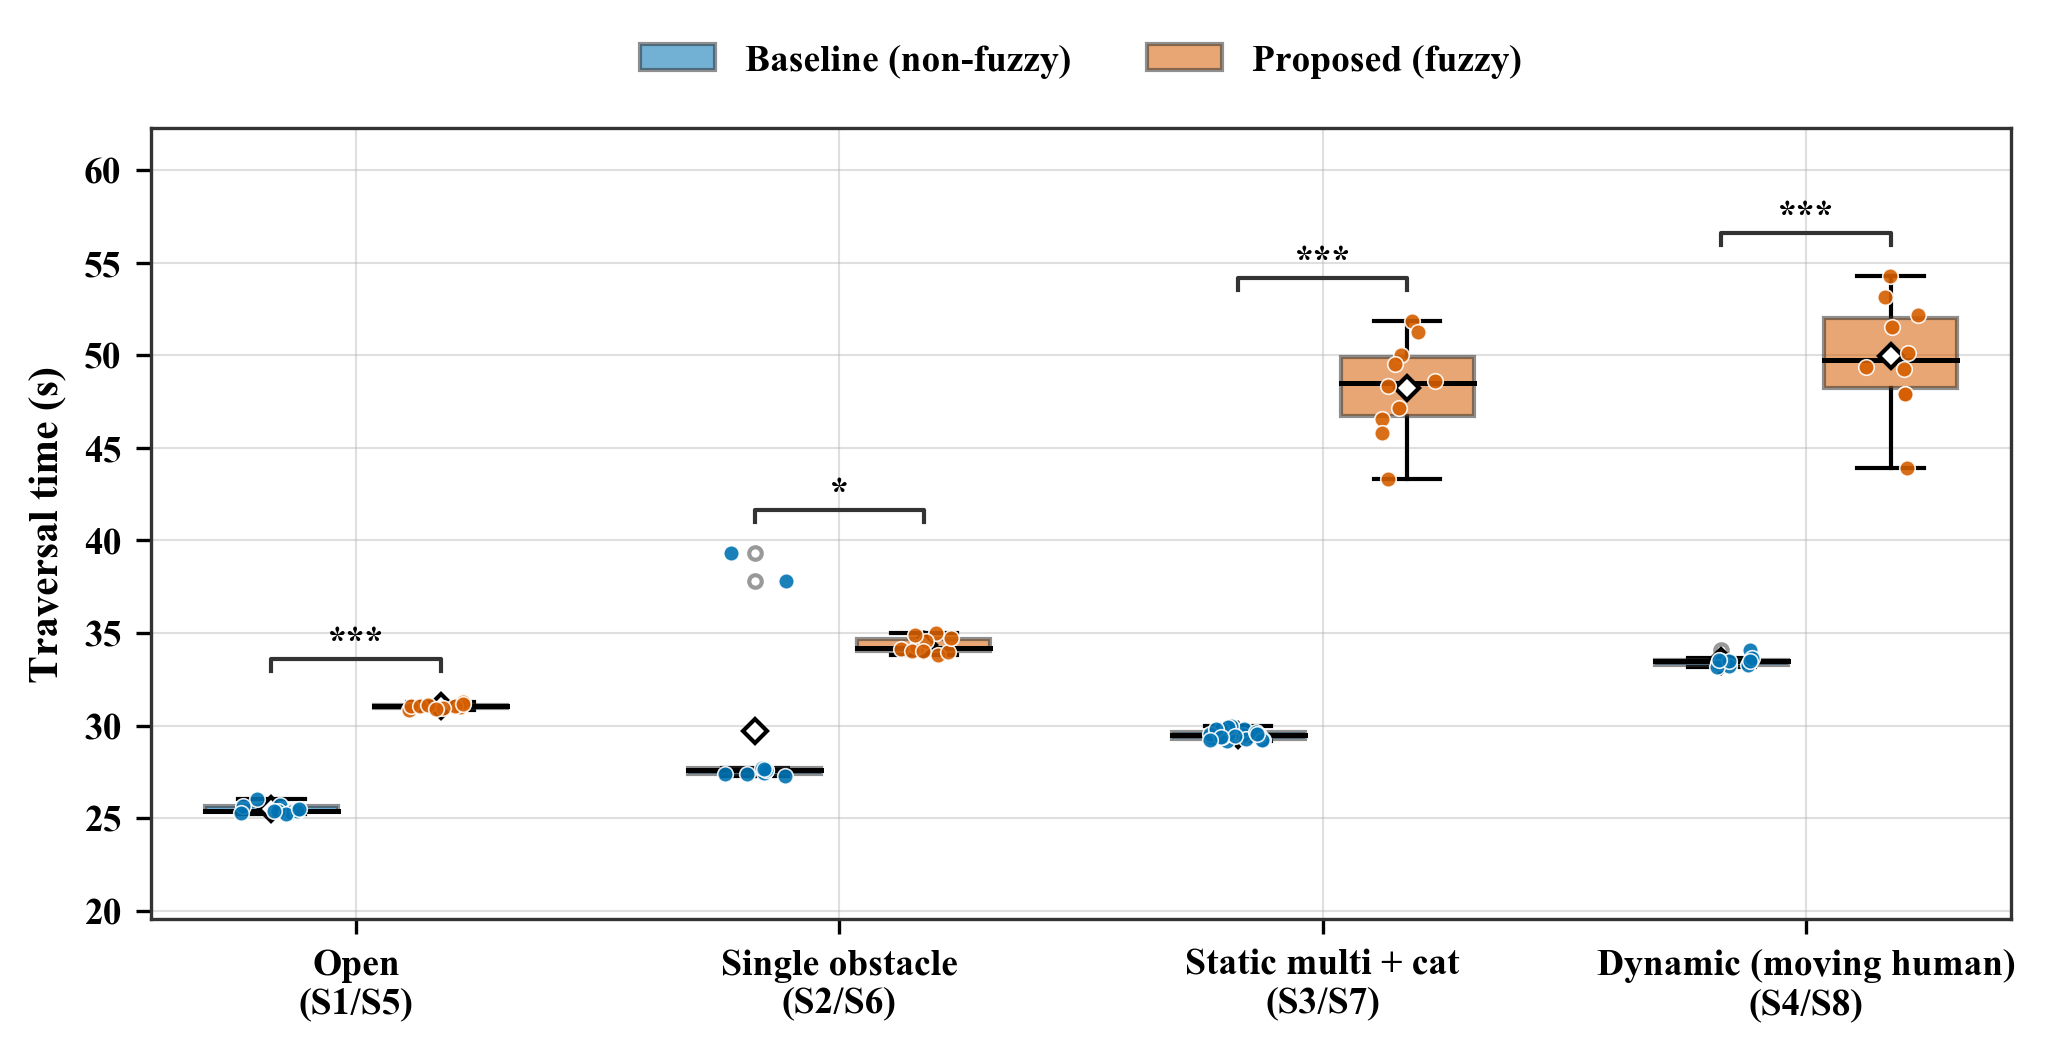
\includegraphics[width=0.6\textwidth]{gambar/fig_time.png}
\caption{Perbandingan waktu tempuh antara konfigurasi baseline dan fuzzy pada seluruh pasangan skenario.}
\label{fig:traversal_time_compare}
\end{figure}

Secara umum terlihat bahwa konfigurasi fuzzy menghasilkan waktu tempuh yang lebih tinggi dibandingkan konfigurasi baseline pada seluruh pasangan skenario. Pada lingkungan terbuka (S1--S5), median waktu tempuh meningkat dari sekitar 25,5 detik menjadi sekitar 31 detik. Peningkatan serupa juga terlihat pada pasangan S2--S6 yang merepresentasikan lingkungan dengan satu obstacle manusia statis.

Perbedaan yang lebih besar muncul pada pasangan S3--S7 dan S4--S8. Pada kedua skenario tersebut, robot dengan konfigurasi fuzzy membutuhkan waktu yang lebih lama untuk mencapai tujuan dibandingkan konfigurasi baseline. Kondisi ini menunjukkan bahwa mekanisme adaptasi fuzzy menyebabkan robot bergerak lebih konservatif ketika mendekati obstacle atau memasuki area dengan nilai traversability yang rendah.

Untuk melihat penyebaran data secara lebih rinci, distribusi waktu tempuh pada setiap skenario divisualisasikan menggunakan boxplot sebagaimana ditunjukkan pada Gambar~\ref{fig:time_boxplot}.

\begin{figure}[H]
\centering
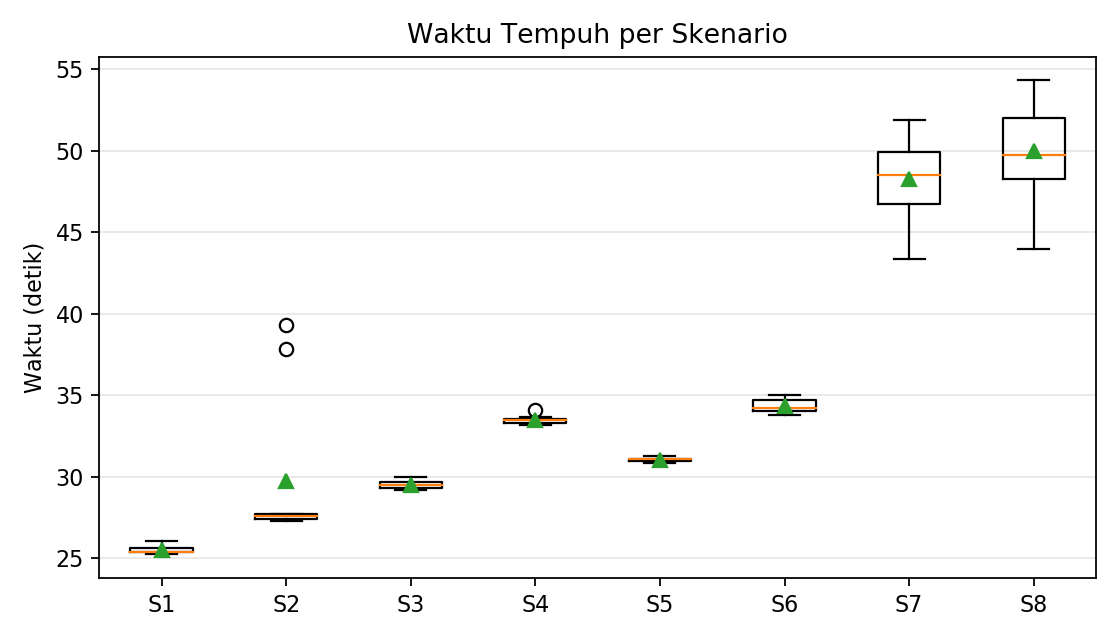
\includegraphics[width=0.6\textwidth]{gambar/fig_time_box.png}
\caption{Distribusi waktu tempuh pada seluruh skenario pengujian.}
\label{fig:time_boxplot}
\end{figure}

Distribusi data menunjukkan bahwa peningkatan waktu tempuh pada konfigurasi fuzzy terjadi secara konsisten pada sebagian besar percobaan. Pada skenario kompleks, khususnya S7 dan S8, peningkatan waktu tempuh sejalan dengan peningkatan \textit{minimum clearance} yang telah dibahas pada Subbab~4.4. Dengan kata lain, robot membutuhkan waktu lebih lama karena mempertahankan jarak aman yang lebih besar terhadap obstacle selama navigasi berlangsung.

Temuan tersebut menunjukkan adanya \textit{trade-off} antara keselamatan dan efisiensi temporal. Mekanisme fuzzy mendorong robot untuk memperlambat pergerakan ketika obstacle berada pada jarak dekat atau ketika nilai traversability lingkungan menurun. Akibatnya, waktu yang dibutuhkan untuk mencapai tujuan meningkat, namun peningkatan tersebut diikuti oleh kenaikan margin keselamatan yang signifikan, terutama pada skenario yang mengandung obstacle berprofil rendah dan obstacle dinamis.

\subsection{Analisis Panjang Lintasan}

Selain waktu tempuh, efisiensi navigasi juga dievaluasi menggunakan panjang lintasan yang ditempuh robot. Metrik ini menggambarkan total jarak yang dilalui robot selama proses navigasi dari titik awal hingga mencapai tujuan.

Distribusi panjang lintasan pada seluruh skenario ditunjukkan pada Gambar~\ref{fig:path_length_boxplot}.

\begin{figure}[H]
\centering
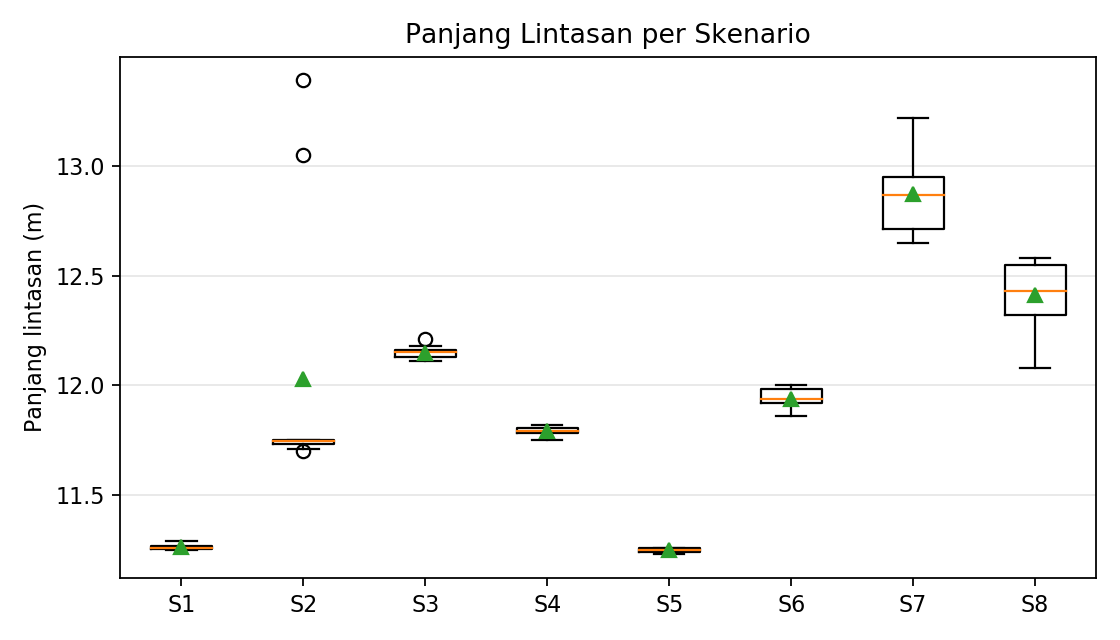
\includegraphics[width=0.6\textwidth]{gambar/fig_path_box.png}
\caption{Distribusi panjang lintasan pada seluruh skenario pengujian.}
\label{fig:path_length_boxplot}
\end{figure}

Hasil pengujian menunjukkan bahwa perbedaan panjang lintasan antara konfigurasi baseline dan fuzzy relatif lebih kecil dibandingkan perbedaan waktu tempuh. Pada lingkungan sederhana, panjang lintasan yang ditempuh kedua konfigurasi cenderung serupa karena robot mengikuti jalur global yang sama dari \textit{NavfnROS}.

Perbedaan mulai terlihat pada lingkungan yang mengandung obstacle berprofil rendah dan obstacle dinamis. Pada konfigurasi fuzzy, robot cenderung mengambil lintasan yang sedikit lebih panjang karena melakukan manuver penghindaran dengan jarak aman yang lebih besar terhadap obstacle. Meskipun demikian, peningkatan panjang lintasan yang terjadi masih berada dalam rentang yang relatif terbatas dibandingkan peningkatan margin keselamatan yang diperoleh.

Hasil ini menunjukkan bahwa peningkatan keselamatan navigasi yang dicapai melalui integrasi kamera termal dan pengendali fuzzy tidak berasal dari perubahan jalur global yang drastis, melainkan dari perubahan perilaku navigasi lokal ketika robot berinteraksi dengan obstacle. Robot tetap mengikuti jalur global yang dihasilkan oleh \textit{NavfnROS}, namun melakukan manuver penghindaran yang lebih konservatif sehingga menghasilkan lintasan yang sedikit lebih panjang.

Dengan mempertimbangkan hasil pada Subbab~4.4, peningkatan panjang lintasan yang terjadi relatif kecil dibandingkan peningkatan margin keselamatan yang diperoleh. Temuan ini mengindikasikan bahwa metode yang diusulkan mampu meningkatkan keselamatan navigasi tanpa menyebabkan degradasi efisiensi lintasan yang signifikan.
